\documentclass[a4paper,11pt,dvipdfmx]{ujarticle}
% パッケージ
\usepackage{graphicx}
\usepackage{url}
% レイアウト指定を記述したファイルの読み込み
\input{layout}

% タイトルと氏名を変更せよ．
\title{日本におけるデジタル化の状況}
\author{G684572026 佐久間 由仁}

\begin{document}

\maketitle %ここにタイトルが入る

% ここから本文
% 節見出し: \section{}
% を使う
\section{ブロードバンドの整備状況}
% 本文(1)
%  参考文献の参照: \cite{}
%  図番号の参照： \ref{}
% を使う
% 文献データベースのキーワードは oecd と imd
% になっている．
OECDによるブロードバンド回線の普及に関する調査\cite{oecd}によると、
図\ref{fig:fig22}に示すように、日本における100人あたりのモバイルブロードバンド
の加入者数は190.5で、第1位になっている。2位はエストニアで、3位米国と続く。
% 図の挿入
% \includegraphics{}
% を
% \begin{figure}[htbp]
% \end{figure}
% で囲み
% \caption{}
% で図のタイトルを入れる．
% \label{}
% を使って図番号が参照できるようにする
% また，
% \centering
% で図が中央に来るようにする
\begin{figure}[htbp]
    \centering
    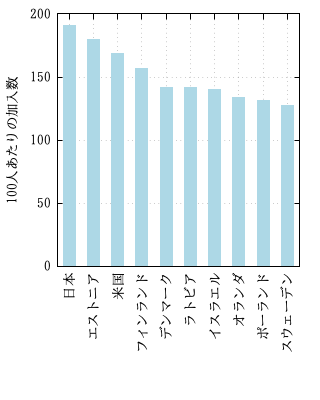
\includegraphics{fig22.png}
    \caption{光ファイバー回線の加入者数（100人あたり）}
    \label{fig:fig22}
\end{figure}
% ーーー
% 節見出し(2)
\section{デジタル競争力ランキング}
% 本文(2)
国際経営開発研究所（IMD）の調査\cite{imd}によると、日本のデジタル競争力のランキングは表\ref{tab:ranking}
に示すように、調査対象の64カ国中、総合で28位、準備性で27位となっている。
% 表の挿入
% \begin{tabular}
% \end{tabular}    
% による表の記述を 
% \begin{table}[htbp]
% \end{table}
% で囲み
% \caption{}
% で表のタイトルを入れる．
% \label{}
% を使って表番号が参照できるようにする
% また，
% \centering
% で表が中央に来るようにする
\begin{table}[htbp]
    \centering
    \caption{デジタル競争力ランキング（64カ国中）}
    \label{tab:ranking}
    \begin{tabular}{|c|c|c|}
        \hline
        国 & 総合 & 準備 \\ \hline
    米国 & 1位 & 1位 \\ \hline
    香港 & 2位 & 10位 \\ \hline
    スウェーデン & 3位 & 6位 \\ \hline
    デンマーク & 4位 & 2位 \\ \hline
    シンガポール & 5位 & 11位 \\ \hline\hline
    韓国 & 12位 & 5位 \\ \hline
    中国 & 15位 & 17位 \\ \hline\hline
    日本 & 28位 & 27位 \\ \hline
    \end{tabular}
\end{table}
% ーーー
% 見出し(3)
% 考察
\section{考察}
% \begin{itemize}
% \end{itemize}
% を使って箇条書きで記述する
\begin{itemize}
    \item 日本は通信インフラは十分に普及していると考えられる。
    \item 日本は活用、実践において他の国に劣っていると考えられる。
    \item よって、日本はもっと技術力を磨くべきだと考えられる。
\end{itemize}
% ここに参考文献が入る
%
\bibliographystyle{junsrt}
\bibliography{exercise.bib}

\end{document}